\section{Numerical Results}
\label{sec:results}

In this section, we provide a representative problem  and amend it to the viscous HJI PDE~\eqref{eq:HJ-RCBRT} to test and verify our hypothesis.

\subsection{The Rockets Launch Problem}
\label{subsec:rockets_launch}
%
We consider the rocket launch problem of Dreyfus~\citet{Dreyfus1966} which was amended to a differential game between two identical rockets, $\pursuer$ and $\evader$, on an $(x,z)$ cross-section of a Cartesian plane in~\citet{levpyconf, LevelSetTOMS}. We want to compute  the usable part~\citet{Isaacs1965} or RCBRT~\citet{Mitchell2005} of the \textit{approximate} terminal surface's boundary for a predefined target set over a target tube.  The usable part entails the regions of the state-space for which the min-max operation over either strategy of $\pursuer$ and $\evader$ is below zero and where the boundary of the usable part (BUP) constitute where \eqref{eq:HJI-RCBRAT} is exactly zero.   

\begin{figure}[t!]
		\includegraphics[width=0.48\textwidth]{../../Safety/DDPReach/figures/rocket/rocket.pdf} 
		\hfill 
		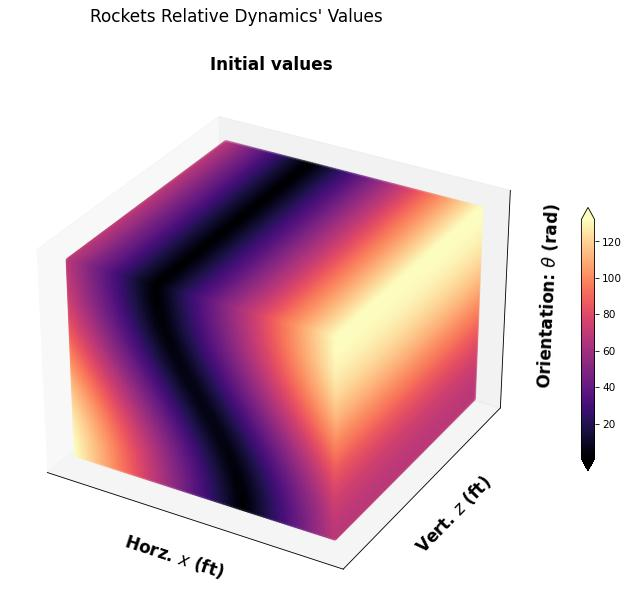
\includegraphics[width=0.48\textwidth]{figures/init_values.jpg} 
	\footnotesize{\caption{\textit{Left:} Motion of two rockets on a Cartesian $\bm{xz}$-plane with a thrust inclination in relative coordinates given by $\theta:=u_p- u_e$. \textit{Right:} Representation of the initial values as a heat map for the two rockets described in \eqref{eq:rocket_spatial_bounds}.}}
	\label{fig:rocket_relative}
\end{figure}
%
For a two-player differential game, let $\pursuer$ and $\evader$ share identical dynamics in a general sense so that we can freely choose the coordinates of $\pursuer$; however, $\evader$'s origin is a distance $\payoff$ away from $(x,z)$ at plane's origin (see Fig. \ref{fig:rocket_relative}) so that the $\pursuer\evader$ vector's inclination measured counterclockwise from the $\state$ axis is $\theta$. 

Hence, we may consider the current problem as a terminal pursuit-evasion \textit{differential} game, whereupon the game terminates when \textit{capture} occurs.  This eventual terminal represents the final \textit{overapproximated} (non)-capture surface for the $\pursuer-\evader$ game (to be shortly introduced). We desire that every \texttt{max} and \texttt{min} operations during a \textit{game of kind} are in the interior of the plane where motion exists; this way, no sudden changes from extremes are too aggravating in cost. 

Let the states of $\pursuer$ and $\evader$  be  $(\state_p, \state_e)$, respectively, driven by thrusts $(u_p, u_e)$ respectively  (see Figure \ref{fig:rocket_relative}). Fix the rockets' range so that what is left of the motion of either $\pursuer$ or $\evader$'s  is restricted to orientation on the $(x,{z})$ plane as illustrated in \autoref{fig:rocket_relative}. 
%
\noindent where $a$ and $g$ are respectively the acceleration and gravitational accelerations (in feet per square second) \footnote{We set $a=1 ft/sec^2$ and $g=32 ft/sec^2$ in our simulation.}.  
As long as $\evader$  remains within this target region or \textit{backward reachable tube} (or BRT), $\pursuer$ cannot cause damage or exercise an action of deleterious consequence on, say, the territory being guarded by $\evader$. Setting up $\evader$ to maximize a payoff quantity  with the largest possible margin or at least frustrate the efforts of $\pursuer$ with minimal collateral damage while the pursuer minimizes this quantity constitutes a terminal value \textit{optimal} differential game: there is no optimal pursuit without an optimal evasion. % since $\pursuer$ and $\evader$ are both executing motions as they see fit within the problem parameters. 

The motion of $\pursuer$  relative to $\evader$'s  along  the $(\state,\bm{z})$ plane includes the relative orientation, the control input, shown in \autoref{fig:rocket_relative} as $\theta=u_p- u_e$. Following the conventions in \autoref{fig:rocket_relative}, the game's relative equations of motion in \textit{reduced space}~\citet[\S 2.2]{Isaacs1965} was derived as (see~\citet[\S VI.A]{levpyconf})
is $\bm{x} = (x, {z}, {\theta})$ where ${\theta }\in \left[-\frac{\pi}{2}, \frac{\pi}{2}\right)$ and $(x,z) \in \bb{R}^2$ are 
%
%{subequations}
%\begin{align}
%\dot{\state} = 
%\begin{cases}
%\dot{x} &= a_p \cos \theta + u_e x, \\
%\dot{z} &=a_p \sin \theta + a_e + u_e x - g, \\%\\
%\dot{\theta} &= u_p -u_e.
%\end{cases}
%\label{eq:rocket_me}
%\end{align}
%\end{subequations}
%
\begin{align}
	\dot{\state} \implies \{ 
		\dot{x} = a_p \cos \theta + u_e x, \,\,
		\dot{z} =a_p \sin \theta + a_e + u_e x - g, \, \, %\\
		\dot{\theta} = u_p -u_e.
		\}
	\label{eq:rocket_me}
\end{align}

The capture radius of the origin-centered circle $\payoff$ (we set $\term=1.5$ ft) is $\|\pursuer \evader\|_2 $ so that $\term^2 =  x^2 + z^2.$
%
All capture points are specified by  the variational HJ PDE~\citet{Mitchell2005}:
%
\begin{align}
\dfrac{\partial \valuefunc}{\partial t} (\bm{x},t) + \min \left[0, \hamfunc\bigg(\state, \frac{\partial \term(\state, t)}{\partial \state}\bigg)\right] \le 0,
\label{eq:rockets_hji}
\end{align}
%
with Hamiltonian given by
%
\begin{align}
\hamfunc(\state, p) &= -\max_{u_e \in [\underline{u}_e, \bar{u}_e]} \min_{u_p \in [\underline{u}_p, \bar{u}_p].
} \begin{bmatrix}
p_1 & p_2 & p_3
\end{bmatrix} 
%
\begin{bmatrix}
a_p \cos \theta + u_e x \\
a_p \sin \theta + a_e + u_p x - g \\
u_p -u_e
\end{bmatrix}.
\label{eq:ham_def}
\end{align}
%
Here,  $p$ are the co-states, and $[\underline{u}_e, \bar{u}_e]$ denotes extremals that the evader must choose as input in response to the extremal controls that the pursuer plays \ie $[\underline{u}_p, \bar{u}_p]$. 
%
Rather than resort to analytical \textit{geometric reasoning}, we may analyze possibilities of behavior by either agent via a principled numerical simulation. This is the essence of this work. 
From \eqref{eq:ham_def}, set $\underline{u}_e = \underline{u}_p = \underline{u} \triangleq -1$ and $\bar{u}_p = \bar{u}_e = \bar{u} \triangleq +1$ so that $\hamfunc(\state, p)$ is
%
\begin{align}
& -\max_{u_e \in [\underline{u}_e, \bar{u}_e]} \min_{u_p \in [\underline{u}_p, \bar{u}_p]
} 
\begin{bmatrix}
p_1(a_p \cos \theta + u_e x) + \nonumber \\ p_2 (a_p \sin \theta + a_e + \nonumber \\ u_p x - g) + p_3 (u_p -u_e)
\end{bmatrix} \nonumber \\
%
%&= -a_p p_1 \cos \theta - a p_2 \sin \theta - a p_2 + g p_2 -\max_{u_e \in [\underline{u}_e, \bar{u}_e]} \min_{u_p \in [\underline{u}_p, \bar{u}_p]} \left(p_1 u_e + p_2 u_p x + p_3 (u_p - u_e)\right), \nonumber \\
%%
%&= -a_p p_1 \cos \theta - a p_2 \sin \theta - a p_2 + g p_2 -\bar{u} |p_1 x +  p_3 | + \underline{u} |p_2 x + p_3 |,  \nonumber \\
%
&\triangleq -a p_1 \cos \theta - p_2 (g - a - a\sin \theta) -\bar{u} |p_1 x +  p_3 |  + \underline{u} |p_2 x + p_3 |,
\label{eq:rocket_hamfunc}
\end{align}
%
where the last line follows from setting $a_e = a_p \triangleq a$. Thus, the rockets HJI equation~\eqref{eq:rockets_hji} becomes
%
\begin{align}
{\partial_t \valuefunc} (t; \bm{x}) + \min \left[0, (-a p_1 \cos \theta - p_2 (g - a - a\sin \theta) -  |p_1 x +  p_3 |  -|p_2 x + p_3 |)\right] \le 0,
\end{align}
%
where $p_1, p_2, p_3$ are the coefficients of the co-states obtained from \eqref{eq:hji_prox_pre}. A similar derivation can be obtained for the \eqref{eq:HJI-RCBRAT}. The initial values of the game is as illustrated in \autoref{fig:initial_values}.


\subsection{Numerical Integration Considerations}
We take the infinitesimal physics problem above and make it algorithmic first by discretizing the spatial and  temporal domains \ie 
%
\begin{align}
	(x, z) \in (-100, +100], \, {\theta} \in (-\pi/2, \pi/2], \,  t \in (0, 1],
	\label{eq:rocket_spatial_bounds}
\end{align}
 %
with $1000$  points along the temporal dimension and $\state_k - \state_{k-1}=1/100$ along the spatial dimensions, where $k \in \mathbb{N}$. All our codes are implemented in pytorch, that runs on an Azure Linux node with the cpu processor specification: Intel Xeon Silver 4208 at 2.1GHz and 65GB memory; The pytorch runs on a Ubuntu 22.04 operating system. 

We defined the target set as the top-left corner of the state space~\autoref{fig:initial_values}  and then run the Algorithm \ref{alg:rcbrt-sample} on a time range of $(0, 1]$ seconds; we chose Dirichlet boundary conditions
%
\begin{align}
	\bm{v}^\delta(0; \bm{x}) = \bm{g}(0; \bm{x}) \triangleq 0.
	\label{eq:rockets_dirichlet}
\end{align} 
%
The spatial gradients (co-states) were computed using the transformation \eqref{eq:prox_value_grad} which were then used in generating the Hamiltonian and subsequently the solution to the safe set using \eqref{eq:rockets_hji}. %In computing the values of the states in \eqref{eq:rocket_me} needed for computing the distance to the target region, we leverage the Runge-Kutta 45 ode integrator~\citet{}
 
% Care is taken not to combine the state components into one full spatial domain early on in the algorithm. We first sampled from each spatial component of \eqref{eq:rocket_spatial_bounds}, compute the values within the expectations in \eqref{eq:prox_value_grad}, and then compute the proximal for the full state space using the expectation-maximization algorithm~\citet{ExpectationMaximization}. The expectation-maximization algorithm proceeded as follows:
% %
% \begin{itemize}
% 	\item We first computed the logarithm of the observations
% \end{itemize} 
% 
% We do not employ a mesh or grid since the indices from which we sample are uniform across $x, z$ and $\theta$. The innards of the expression in \eqref{eq:prox_value_grad}  were first computed based on samples from the state space \eqref{eq:rocket_spatial_bounds}. %The expectation from the Gaussian distributions are computed with the expectation-maximization algorithm~\citet{JordanExpectimax}. %which yielded the proximal expression in terms of the spatial gradient of the value function.